\documentclass{article}
\usepackage{ctex}
\usepackage{geometry}
\geometry{a4paper, scale=0.8}
\usepackage{graphicx}
\usepackage{float}
\usepackage{enumitem}
\usepackage{amsmath}
\usepackage{amssymb}
\usepackage{multirow}
\usepackage{makecell}
\usepackage{subfigure}
\usepackage{fontspec}
\newfontfamily\jetbrains{JetBrains Mono}
\usepackage{listings}
\usepackage{color}
\lstset{
    breaklines,                                 % 自动将长的代码行换行排版
    extendedchars=false,                        % 解决代码跨页时,章节标题,页眉等汉字不显示的问题
    backgroundcolor=\color[rgb]{0.96,0.96,0.96},% 背景颜色
    keywordstyle=\color{blue}\bfseries,         % 关键字颜色
    identifierstyle=\color{black},              % 普通标识符颜色
    commentstyle=\color[rgb]{0,0.6,0},          % 注释颜色
    stringstyle=\color[rgb]{0.58,0,0.82},       % 字符串颜色
    showstringspaces=false,                     % 不显示字符串内的空格
    numbers=left,                               % 显示行号
    numberstyle=\tiny\jetbrains,                    % 设置数字字体
    basicstyle=\small\jetbrains,                    % 设置基本字体
    captionpos=t,                               % title在上方(在bottom即为b)
    frame=single,                               % 设置代码框形式
    rulecolor=\color[rgb]{0.8,0.8,0.8},         % 设置代码框颜色
}
\usepackage{caption}
\usepackage{hyperref}
\hypersetup{
    hypertex=true,
    colorlinks=true,
    linkcolor=black,
    anchorcolor=black,
    citecolor=black
}


\title{HW01}
\author{PB19071405\ 王昊元}
\date{2022 年 3 月 29 日}

\begin{document}
    \pagestyle{empty}
    \maketitle
    \thispagestyle{empty}

    \begin{enumerate}[label=\arabic*.]
        \item 等价类表如下:(其中认为接种者数字编号从00000开始)\\
        \scalebox{1}
        {
            \begin{tabular}{|c|c|c|c|c|}
                \hline
                功能项 & 有效等价类 & 编号 & 无效等价类 & 编号 \\
                \hline
                \multirow{5}{*}{接种号} & 10位 & 1 & \makecell[c]{少于10位(包括空) \\ 多于10位} & \makecell[c]{2 \\ 3} \\
                \cline{2-5}
                ~ & 首位为A、B或C & 4 & \makecell[c]{D-Z的大写字母 \\ 小写字母 \\ 其他字符} & \makecell[c]{5 \\ 6 \\ 7} \\
                \cline{2-5}
                ~ & 2\textasciitilde 3位为01\textasciitilde 12的数字 & 8 & \makecell[c]{00 \\ 13\textasciitilde 99 \\ 包含其它字符} & \makecell[c]{9 \\ 10 \\ 11} \\
                \cline{2-5}
                ~ & 4\textasciitilde 5位为07、13或23 & 12 & \makecell[c]{00\textasciitilde 06 \\ 08\textasciitilde 12 \\ 14\textasciitilde 22 \\ 24\textasciitilde 99 \\ 包含其它字符} & \makecell[c]{13 \\ 14 \\ 15 \\ 16 \\ 17} \\
                \cline{2-5}
                ~ & 6\textasciitilde 10位为数字 & 18 & 包含其它字符 & 19 \\
                \hline
            \end{tabular}
        }

        覆盖数据如下: \\
        \scalebox{0.8}
        {
            \begin{tabular}{|c|c|c|c|p{0.5\textwidth}|}
                \hline
                序号 & 输入数据 & 覆盖等价类 & 预期输出 & 备注 \\
                \hline
                1 & C030700000 & 1、4、8、12、18 & 合法输入 & ~ \\
                \hline
                2 & C03070000 & 2、4、8、12 & 非法输入 & 因最后不足5位,故不认为覆盖第18号等价类 \\
                \hline
                3 & C0307000000 & 3、4、8、12、18 & 非法输入 & ~ \\
                \hline
                4 & F030700000 & 1、5、8、12、18 & 非法输入 & ~ \\
                \hline
                5 & c030700000 & 1、6、8、12、18 & 非法输入 & ~ \\
                \hline
                6 & >030700000 & 1、7、8、12、18 & 非法输入 & ~ \\
                \hline
                7 & C000700000 & 1、4、9、12、18 & 非法输入 & ~ \\
                \hline
                8 & C130700000 & 1、4、10、12、18 & 非法输入 & ~ \\
                \hline
                9 & CAB0700000 & 1、4、11、12、18 & 非法输入 & ~ \\
                \hline
                10 & C030400000 & 1、4、8、13、18 & 非法输入 & ~ \\
                \hline
                11 & C031100000 & 1、4、8、14、18 & 非法输入 & ~ \\
                \hline
                12 & C032100000 & 1、4、8、15、18 & 非法输入 & ~ \\
                \hline
                13 & C039900000 & 1、4、8、16、18 & 非法输入 & ~ \\
                \hline
                14 & C03AB00000 & 1、4、8、17、18 & 非法输入 & ~ \\
                \hline
                15 & C03070000A & 1、4、8、12、19 & 非法输入 & ~ \\
                \hline
            \end{tabular}
        }
        
        \item \ \begin{enumerate}[label=代码\arabic*]
            \item 流图如下所示:\\
            \begin{figure}[H]
                \centering
                % 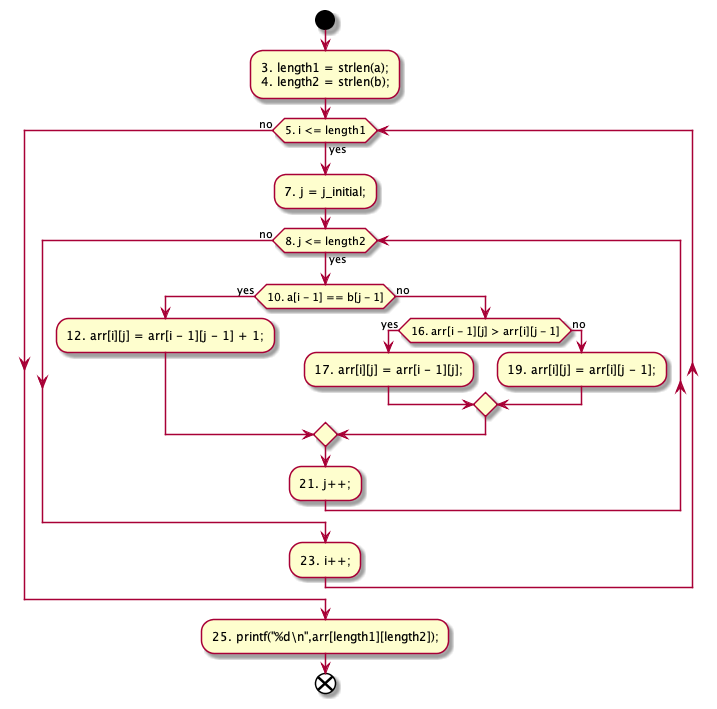
\includegraphics[width=0.7\textwidth]{fig/hw01/flow_diagram1.png}
                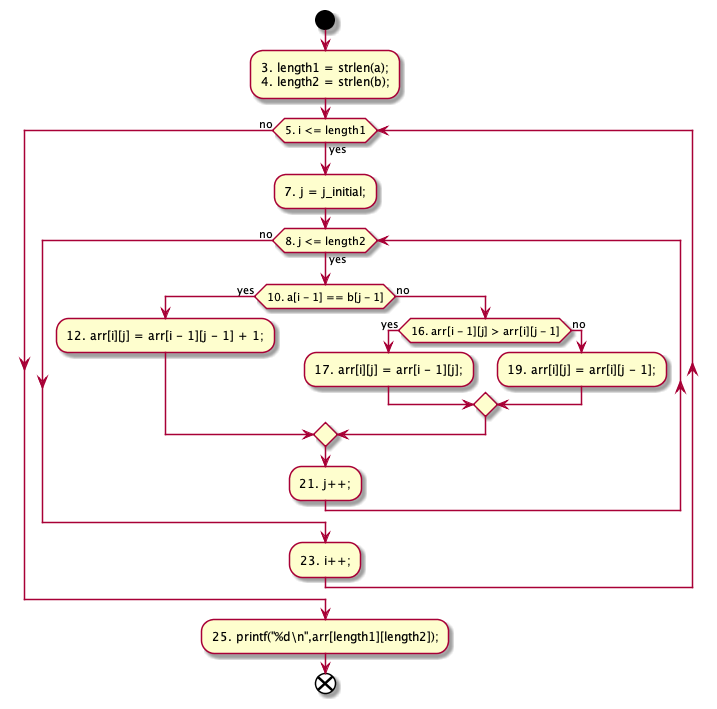
\includegraphics[scale=0.5]{fig/hw01/flow_diagram1.png}
                \caption{代码1流图}
            \end{figure}

            环路复杂度为:$4 + 1 = 5$

            测试用例如下:\\
            \begin{tabular}{|c|c|c|}
                \hline
                独立路径 & 测试用例 & 结果 \\
                \hline
                3,4-5-25 & \verb|i = 10, j_initial = 1, a = "ABCD", b = "BAD"| & 打印0 \\
                \hline
                3,4-5-7-8-23-5-25 & \verb|i = 1, j_initial = 10, a = "ABCD", b = "BAD"|  & 打印0 \\
                \hline
                3,4-5-7-8-10-12-21-8-23-5-25 & \verb|i = 1, j_initial = 1, a = "A", b = "A"| & 打印1 \\
                \hline
                3,4-5-7-8-10-16-17-21-8-23-5-25 & 该路径实际不存在,无测试样例 & ~ \\
                \hline
                3,4-5-7-8-10-16-19-21-8-23-5-25 & \verb|i = 1, j_initial = 1, a = "A", b = "B"| & 打印0 \\
                \hline
            \end{tabular}

            \item 流图如下所示:\\
            \begin{figure}[H]
                \centering
                % 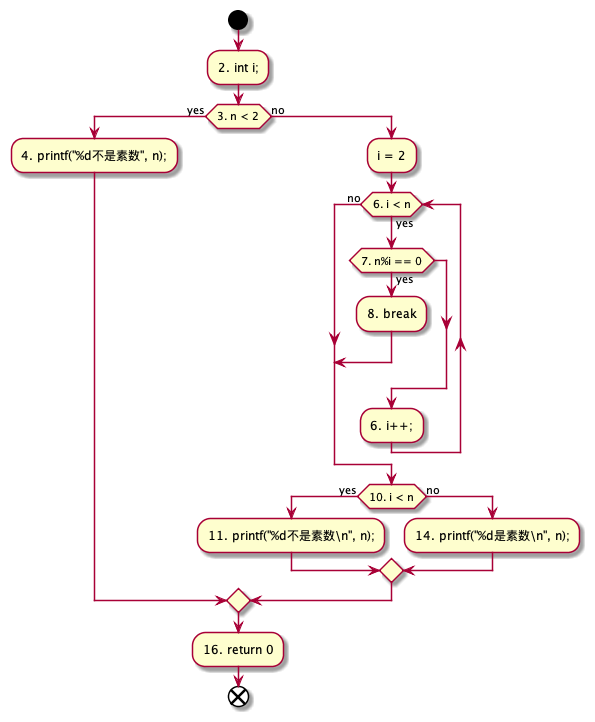
\includegraphics[width=0.7\textwidth]{fig/hw01/flow_diagram2.png}
                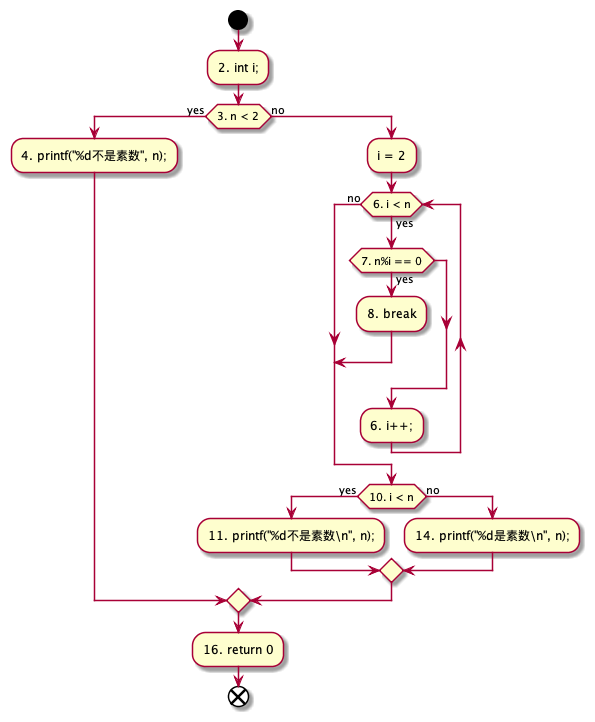
\includegraphics[scale=0.5]{fig/hw01/flow_diagram2.png}
                \caption{代码2流图}
            \end{figure}

            环路复杂度为:$4 + 1 = 5$

            测试用例如下:\\
            \begin{tabular}{|c|c|c|}
                \hline
                独立路径 & 测试用例 & 结果 \\
                \hline
                2,3,4,16 & \verb|n = 1| & 打印1不是素数 \\
                \hline
                2,3,6,10,11,16 & 该路径实际不存在,无测试样例 & ~ \\
                \hline
                2,3,6,10,14,16 & \verb|n = 2| & 打印2是素数 \\
                \hline
                2,3,6,7,6,10,14,16 & \verb|n = 3| & 打印3是素数 \\
                \hline
                2,3,6,7,8,10,11,16 & \verb|n = 4| & 打印4不是素数 \\
                \hline
            \end{tabular}
        \end{enumerate}

        \item 包含不同严重程度bug的python程序 \\
        \begin{lstlisting}[language=python]
class MyException:
    def __init__(self, msg):
        print(msg)
        return self

def foo(s: str, l: int):
    l = 10
    try:
        if l == 0:
            print("no string?")
        elif l > 0:
            print("The length of string \"{}\": {}".format(s, l))
        elif l == 0:
            print("?")
        else:
            raise MyException("length is negative.")
    except Exception as e:
        pass
    msg = s + l
    print(msg)
    return
    ++l
    print("The result of code \"++l\": {}".format(l))
    break
    print("function foo done.")

s = "PB19071405"
foo(s, 5)

        \end{lstlisting}
        SonarQube检测结果如下:\\
        \begin{figure}[H]
            \centering
            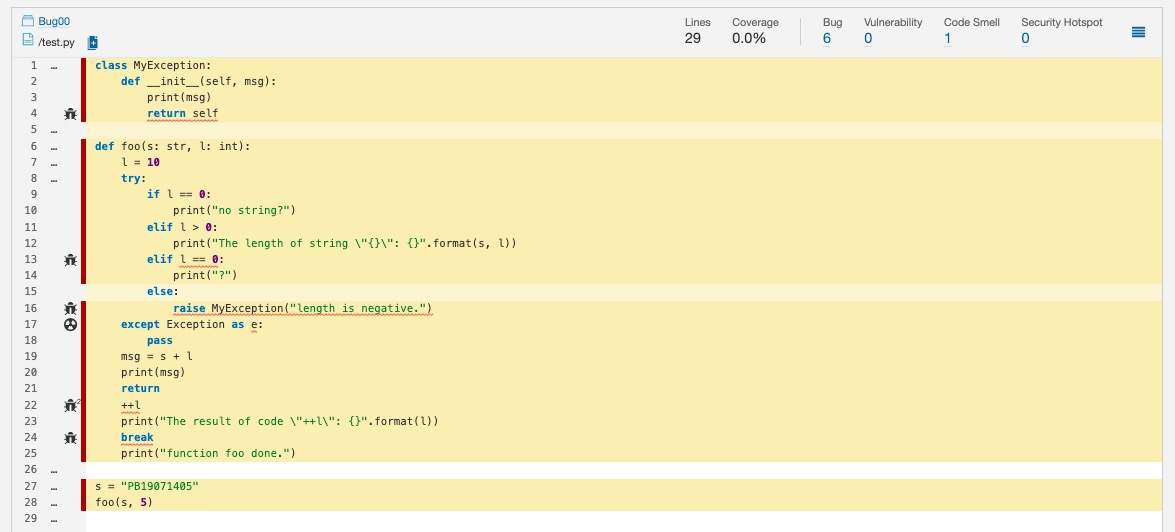
\includegraphics[width=0.7\textwidth]{fig/hw01/all_code.jpg}
            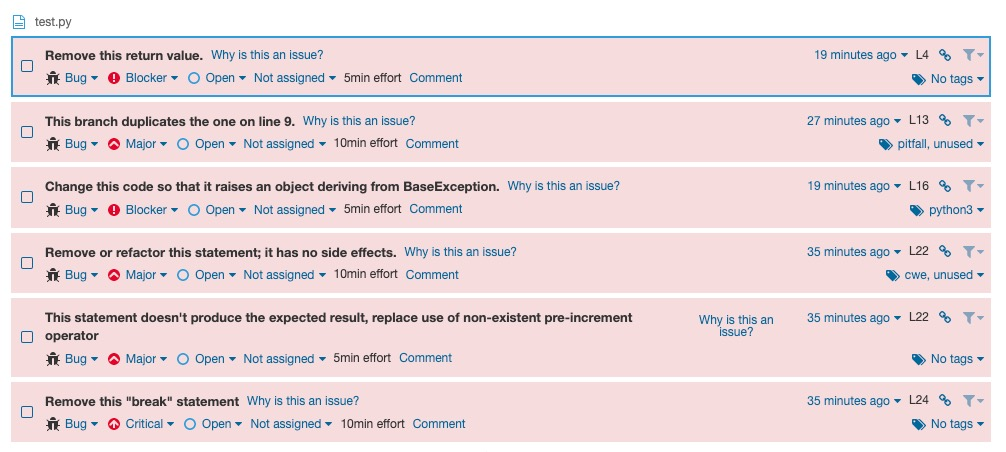
\includegraphics[width=0.7\textwidth]{fig/hw01/all_bug.jpg}
            \caption{完整代码及检测出的bug}
        \end{figure}
        \begin{figure}[H]
            \centering
            \subfigure[Function parameters initial values should not be ignored]{
                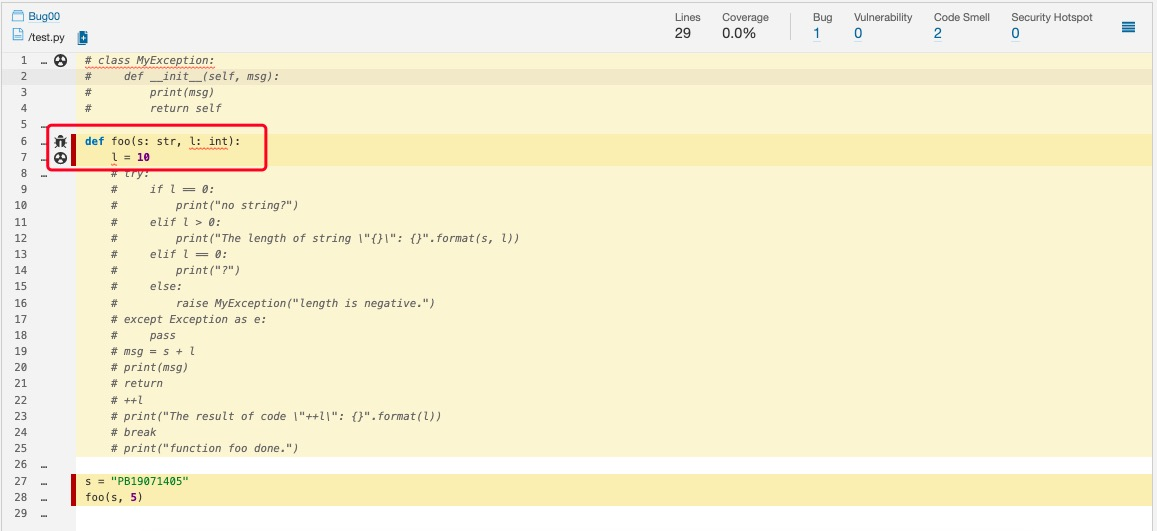
\includegraphics[width=0.7\textwidth]{fig/hw01/param_bug.jpg}
            }\\
            \subfigure[All code should be reachable]{
                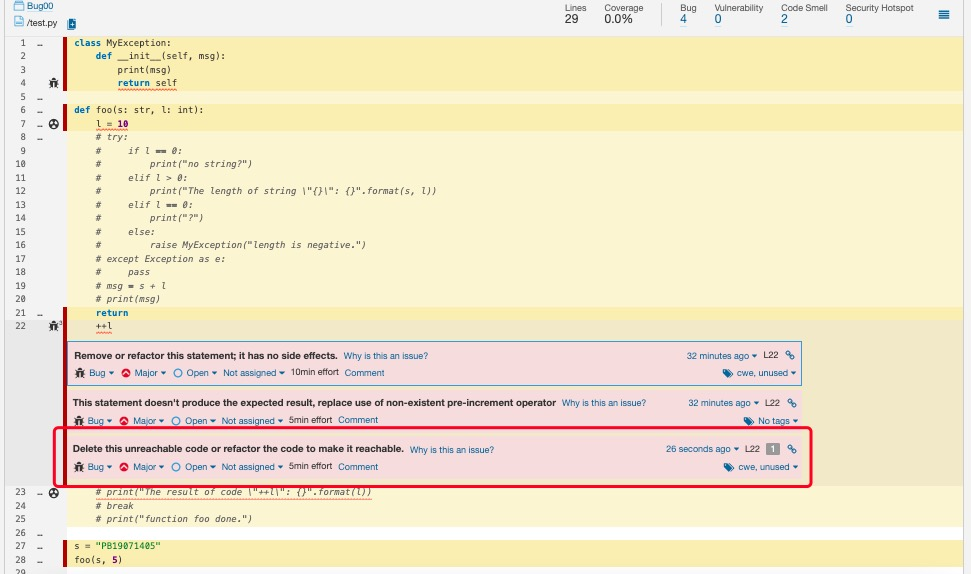
\includegraphics[width=0.7\textwidth]{fig/hw01/reachable_bug.jpg}
            }
            \caption{一些在完整代码中没有被检测出的bug}
        \end{figure}

        修复后的代码如下(修改方案及原因由对应注释说明):\\
        \begin{lstlisting}[language=python]
# Raised Exceptions must derive from BaseException
# 修复方案:将 MyException 类继承于 BaseException
class MyException(Exception):
    def __init__(self, msg):
        print(msg)
        # "__init__" should not return a value
        # __init__()函数应返回 None
        # 修复方案:不 return 或 return None

        # return self
        return None

def foo(s: str, l: int):
    # Function parameters initial values should not be ignored
    # 根据官方说明,这种行为只是像一个bug,
    # 因为参数传进来的值并没有用,设置的参数也就失去了意义
    # 但实际coding过程中可能很少会出现这个bug
    # 修复方案:直接注释/删除掉
    # 注:本来打算通过修改变量名的方式来修复这个bug,
    # 但考虑到修改变量名会产生 Unused local variables should be removed 的 Code Smell,
    # 最后决定通过注释/删除来修复

    # l = 10
    try:
        if l == 0:
            print("no string?")
        elif l > 0:
            print("The length of string \"{}\": {}".format(s, l))
        # Related "if/else if" statements should not have the same condition
        # 实际coding过程中也很少遇到,
        # 但是不排除太多种情况用if/else if实现时脑袋混乱最后导致该bug的情况
        # 修复方案:注释/删除一个分支即可

        # elif l == 0:
        #     print("?")
        else:
            # Raised Exceptions must derive from BaseException
            # 该bug实际报错在此处,因为只有解释该语句时才会发现这个没有继承自 BaseException 的类被 raise 了
            # 修复方案:修改 MyException 继承自 BaseException
            raise MyException("length is negative.")
    except Exception as e:
        # 其实这个地方应该有一个 Unused local variables should be removed 的 Code Smell 来着(以我个人的理解),
        # 但是没有出现。事实上我个人的习惯是将 Exception 打印出来,也方便 debug
        # 修复方案:使用变量 e (如:print(e))

        # pass
        print(e)
    # Operators should be used on compatible types
    # 不过应该是因为在定义函数的时候其实并不知道 s 和 l 的类型,所以没检测出来这个 Blocker 的 bug
    # 修复方案:可以通过try - except 解决
    # 但其实平时也只会在有可能产生 Exception 的地方加 try,或者在函数刚开始的时候进行变量类型的检查之类的
    try:
        msg = s + l
        print(msg)
    except Exception as e:
        print(e)
    # All code should be reachable
    # 修复方案:删除/注释 return

    # return

    # Increment and decrement operators should not be used
    # 修复方案:删除/注释
    # ++l
    print("The result of code \"++l\": {}".format(l))
    # "break" and "continue" should not be used outside a loop
    # 修复方案:删除 break
    # break
    print("function foo done.")

s = "PB19071405"
foo(s, 5)

        \end{lstlisting}

        修复后进行测试,结果如下:\\
        \begin{figure}[H]
            \centering
            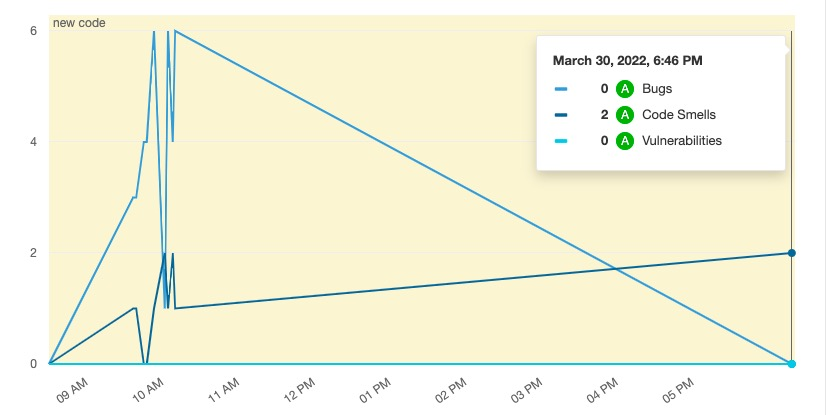
\includegraphics[width=0.7\textwidth]{fig/hw01/fixed.jpg}
            \caption{修复后的代码及修复方案}
            \label{fixed}
        \end{figure}

        图 \ref{fixed} 中有两个 Code Smells,是由于写修复方案的注释与空格导致的。


    \end{enumerate}

\end{document}
